\chapter{Marco Teórico}

\section{Líquenes}

Los líquenes son organismos simbióticos formados por la asociación entre un hongo y un alga (o cianobacteria). Esta simbiosis les permite colonizar sustratos difíciles, como superficies rocosas y piedras de monumentos arqueológicos, donde otros organismos no podrían sobrevivir. Su capacidad para fijarse en estas superficies los convierte en organismos pioneros en los procesos de colonización biológica. \cite{Gamboa2017}

Sin embargo, la presencia de líquenes en monumentos y construcciones históricas puede ser un factor significativo de biodeterioro. Al crecer sobre la piedra, su talo puede retener humedad que promueve la meteorización física y química, además de provocar la desagregación mineral. Por ello, es crucial entender su biología para diseñar estrategias eficaces de conservación del patrimonio pétreo en centros arqueológicos.

\begin{figure}[h]
	\centering
	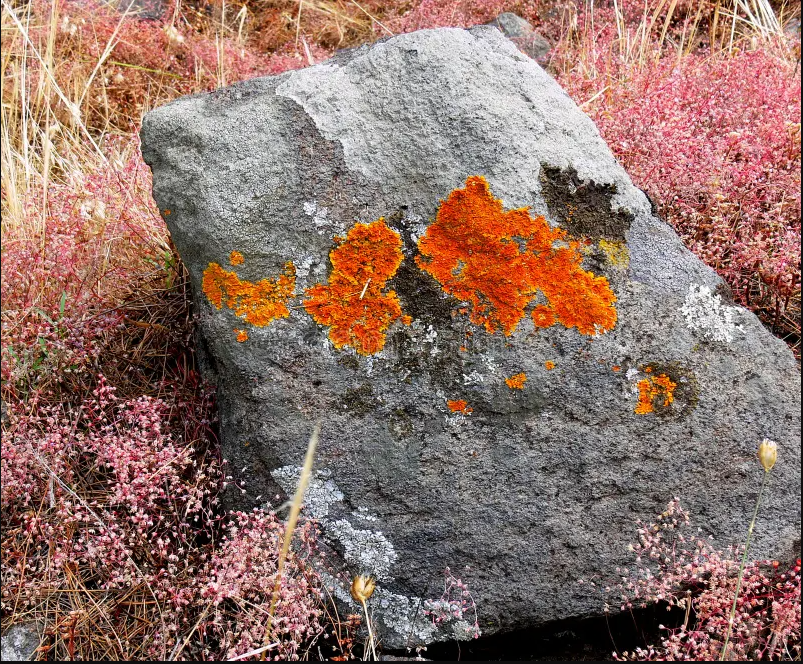
\includegraphics[width=0.5\linewidth]{media/liquen-roca}
	\caption{Organismo Liquen en una roca}
	\label{fig:liquen-roca}
\end{figure}


\section{Cobertura Liquenica}

La cobertura líquenica se refiere a la extensión o superficie ocupada por las colonias de líquenes sobre un sustrato, en este caso, las piedras de monumentos arqueológicos. Un alto nivel de cobertura puede indicar un proceso avanzado de colonización que puede acelerar el deterioro del material.

La cuantificación de la cobertura líquenica es vital para monitorear la integridad de las piedras y evaluar la efectividad de tratamientos conservacionistas. Estos datos permiten identificar zonas críticas donde la acción de los líquenes es más intensa y donde las medidas de conservación deben ser prioritarias para proteger el patrimonio. \cite{Gamboa2017}

\begin{figure}[h]
	\centering
	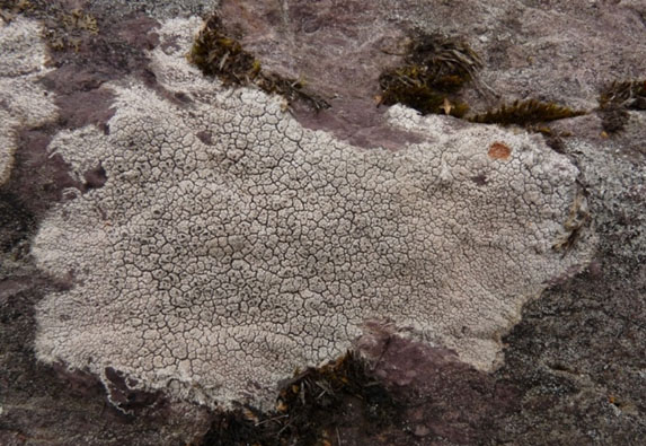
\includegraphics[width=0.5\linewidth]{media/superficie-liquenica}
	\caption{Superficie liquenica - area de ocupación}
	\label{fig:superficie-liquenica}
\end{figure}


\section{Simbiosis liquénica}

La simbiosis líquenica es la relación mutualista entre hongos y algas o cianobacterias que da lugar al organismo visible como líquen. Esta asociación es fundamental para la resiliencia de los líquenes, permitiéndoles sobrevivir en ambientes extremos y colonizar materiales sólidos.

Esta particularidad implica que los líquenes tienen mecanismos adaptativos que favorecen su persistencia sobre las piedras, complicando su eliminación y aumentando el riesgo de biodeterioro en monumentos arqueológicos. Comprender esta simbiosis es clave para desarrollar tratamientos que respeten la estabilidad del monumento mientras controlan el crecimiento del líquen.

\begin{figure}[h]
	\centering
	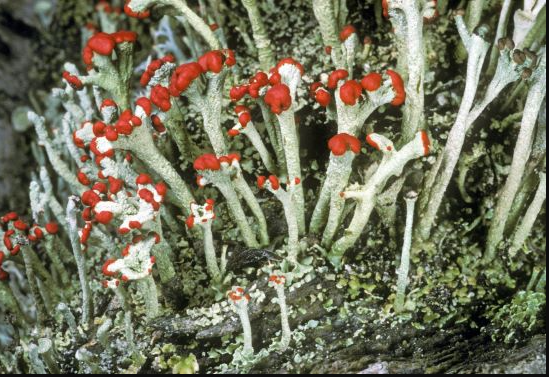
\includegraphics[width=0.5\linewidth]{media/simbiosis-liquenica}
	\caption{Simbiosis entre especies Liquenicas - Liquen - fungica vegetal}
	\label{fig:simbiosis-liquenica}
\end{figure}


\section{Biodeterioro}

El biodeterioro es el proceso de degradación de materiales, en este caso rocas y piedras monumentales, causado por la acción de agentes biológicos como líquenes, hongos, bacterias y musgos. Estos organismos pueden alterar la estructura física y química de las piedras, debilitando su integridad.

En los centros arqueológicos, el biodeterioro representa una amenaza significativa para la conservación a largo plazo del patrimonio pétreo. La acción conjunta de microorganismos favorece la exfoliación, fisuración y cambio de color en las piedras, lo que puede llevar a la pérdida irreversible de información histórica y cultural contenida en los monumentos.

Según se cita de \cite{Gamboa2017}


\section{Patrimonio arqueológico}

El patrimonio arqueológico está constituido por los bienes culturales materiales de valor histórico, tales como monumentos, construcciones y artefactos que representan la herencia de civilizaciones pasadas. Las piedras que conforman estos elementos son testimonios materiales fundamentales para el estudio del pasado.

La conservación del patrimonio arqueológico implica proteger las piedras de la acción degradativa de factores biológicos como los líquenes. Su cuidado es esencial para preservar no solo la integridad física de los monumentos sino también el valor simbólico y cultural que estos representan para las generaciones presentes y futuras.

\begin{figure}[h]
	\centering
	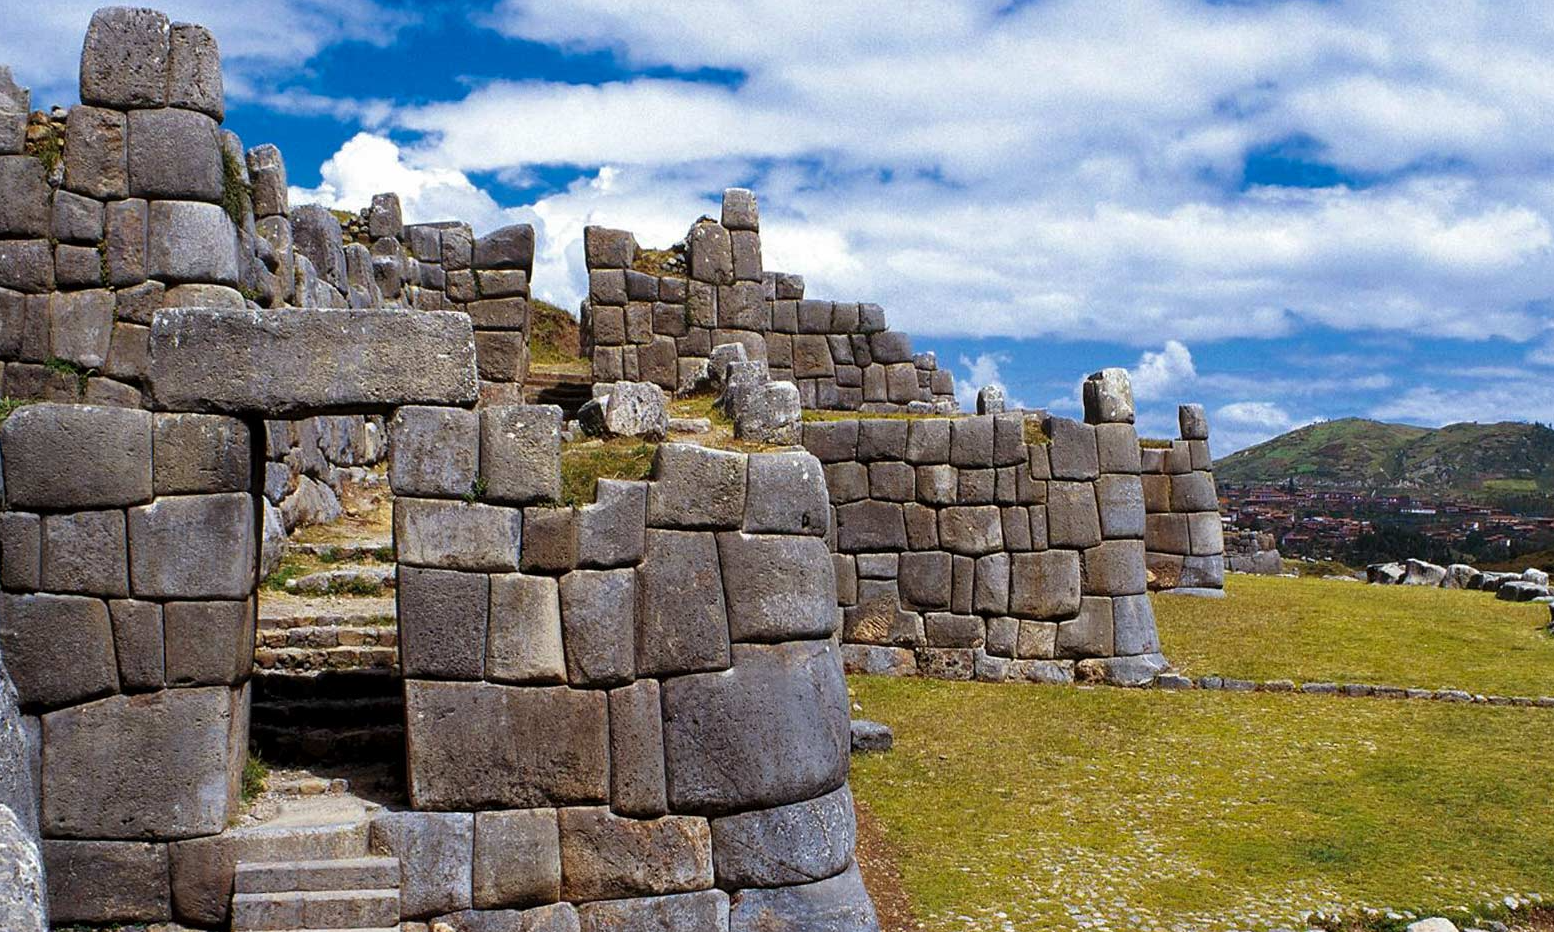
\includegraphics[width=0.5\linewidth]{media/patrimonio-cultural}
	\caption{Patrimonio cultural - Sacsayhuaman Cusco}
	\label{fig:patrimonio-cultural}
\end{figure}


\section{Deterioro pétreo}

El deterioro pétreo es el conjunto de procesos que degradan la piedra, tanto por causas naturales como antropogénicas. Entre las causas naturales destacan la acción del agua, la temperatura, la contaminación atmosférica y la acción biológica como la de los líquenes, que provocan procesos físicos, químicos y biológicos que modifican la estructura y composición del material pétreo.

En contextos arqueológicos, el deterioro pétreo puede ser acelerado tras la excavación, que expone las piedras a condiciones ambientales nuevas. Es fundamental controlar agentes como los líquenes para evitar que el desgaste avance y se pierda información cultural contenida en las piedras.

\begin{figure}[h]
	\centering
	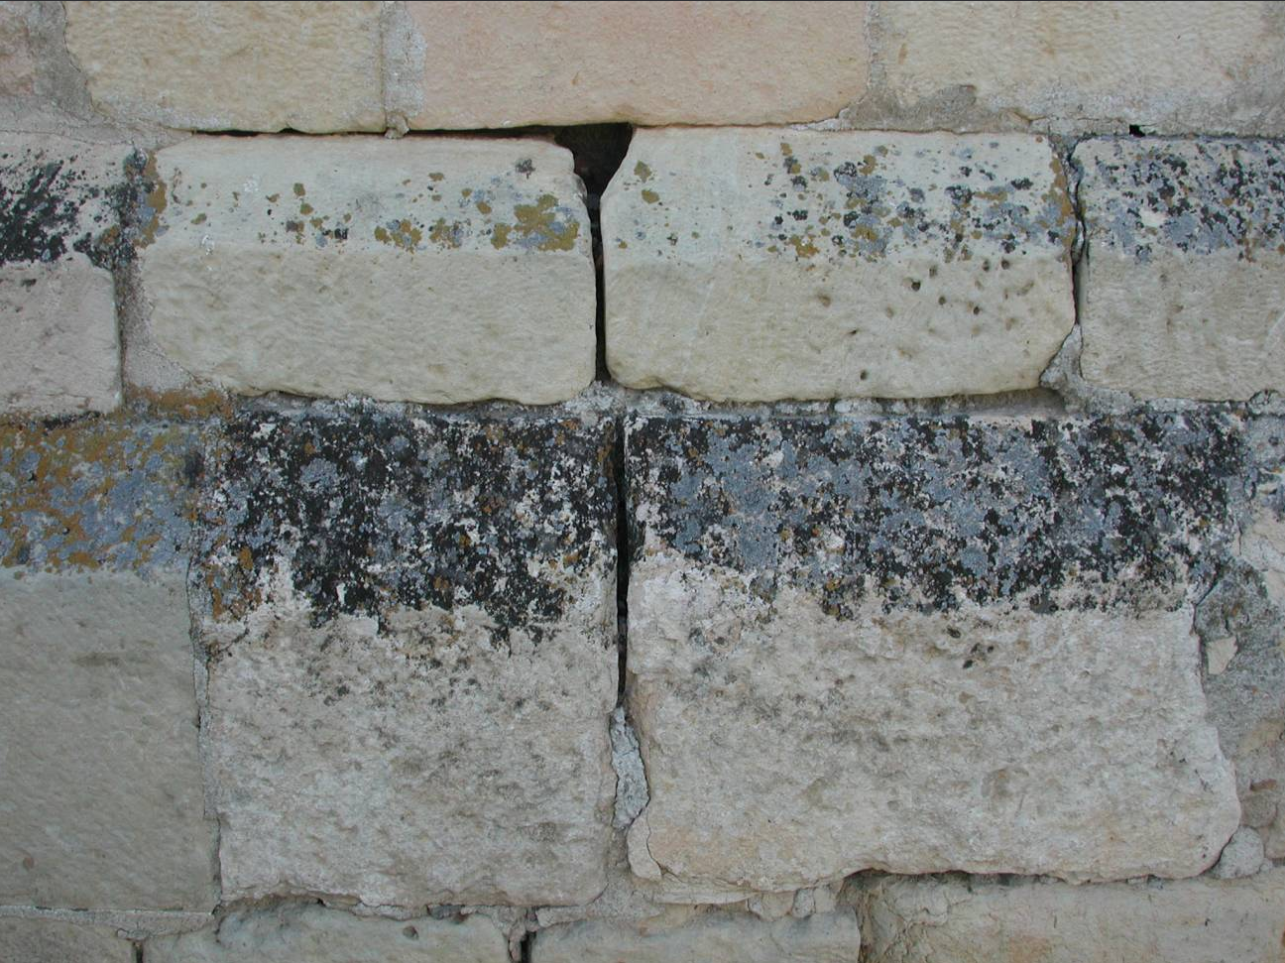
\includegraphics[width=0.5\linewidth]{media/biodeterioro-liquen}
	\caption{Desgaste y/o biodeterioro piedra a causa de los liquenes}
	\label{fig:biodeterioro-liquen}
\end{figure}


Según se cita en \cite{Navarrete2022}

\section{Segmentación de imágenes}

La segmentación de imágenes es una técnica de procesamiento digital que permite separar y clasificar distintas zonas dentro de una imagen, facilitando el análisis específico de áreas afectadas por líquenes en las piedras. Es una herramienta útil para cuantificar la cobertura líquenica de manera objetiva y reproducible. 

Esta técnica es importante para la conservación de monumentos porque posibilita la identificación temprana de zonas deterioradas y el monitoreo continuo del progreso del biodeterioro. Así se pueden tomar decisiones informadas sobre intervenciones conservacionistas y su seguimiento en el tiempo.

\section{Reflectancia espectral}

La reflectancia espectral mide la cantidad de luz que una superficie refleja en diferentes longitudes de onda. En el estudio de líquenes, la reflectancia espectral permite detectar y caracterizar la presencia de estas colonias sobre piedras mediante técnicas remotas o en campo.

Este método es valioso para la conservación porque permite evaluar la extensión y tipo de cobertura líquenica sin contacto físico con el monumento, minimizando daños y facilitando protocolos de monitoreo eficientes y no invasivos para la protección del patrimonio pétreo.

\begin{figure}[h]
	\centering
	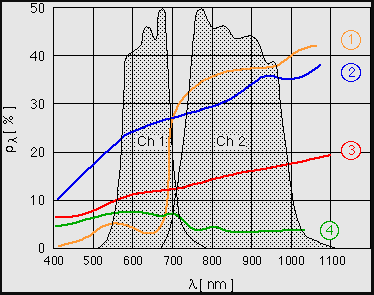
\includegraphics[width=0.5\linewidth]{media/reflectancia-espectral}
	\caption{Reflectancia espectral para determinar el tipo de planta en función a la longitud de onda en la luz reflejada}
	\label{fig:reflectancia-espectral}
\end{figure}


\section{Índices espectrales}

Los índices espectrales son combinaciones matemáticas de reflectancias en diferentes bandas del espectro electromagnético que realzan características específicas de la superficie, como la vegetación o en este caso, la cobertura líquenica. Son herramientas útiles para detectar y cuantificar la presencia de líquenes en imágenes obtenidas por satélites o drones.

Estos índices permiten a los especialistas en conservación identificar patrones de colonización biológica y evaluar el impacto del biodeterioro en áreas arqueológicas. De esta forma, se optimizan las estrategias de conservación mediante un análisis más preciso y global.

\section{Validación de campo}

La validación de campo es el proceso de verificar in situ los datos obtenidos por técnicas remotas o analíticas, calibrando y confirmando la información sobre la presencia y extensión de líquenes en las piedras. Es un paso crucial para garantizar la fiabilidad de los estudios y tratamientos de conservación.

Esta validación es fundamental en centros arqueológicos porque asegura que las medidas de monitoreo y control del biodeterioro basadas en tecnologías avanzadas coinciden con la realidad física, permitiendo así intervenciones más efectivas y acertadas para preservar los monumentos.

